% DATA_SHA256: f8b2319e245f60439f4a47ebf2fc63d77cf12c4ed7e72c3c62a845b4a2ae7033
\documentclass[tikz,border=6pt]{standalone}
\usepackage[T1]{fontenc}
\usepackage{helvet}
\renewcommand{\familydefault}{\sfdefault}
\usetikzlibrary{arrows.meta,positioning,fit,backgrounds,calc,shapes.geometric}
% Native TikZ style for ATLAS SERS plan figures. No raster assets.
\definecolor{oiBlue}{HTML}{0072B2}
\definecolor{oiSky}{HTML}{56B4E9}
\definecolor{oiGreen}{HTML}{009E73}
\definecolor{oiOrange}{HTML}{E69F00}
\definecolor{oiVermillion}{HTML}{D55E00}
\definecolor{oiPurple}{HTML}{CC79A7}
\definecolor{oiYellow}{HTML}{F0E442}
\definecolor{softGray}{HTML}{F3F5F7}
\tikzset{
  planbox/.style={draw=black!70, rounded corners=2pt, line width=.65pt,
    align=center, minimum height=10mm, text width=34mm, font=\sffamily\footnotesize,
    inner sep=4pt},
  foundation/.style={planbox, fill=oiSky!20},
  modeling/.style={planbox, fill=oiOrange!22},
  evaluation/.style={planbox, fill=oiGreen!17},
  synthesis/.style={planbox, fill=oiPurple!17},
  gate/.style={diamond, aspect=2.15, draw=black!75, fill=oiYellow!45,
    line width=.7pt, align=center, font=\sffamily\scriptsize, inner sep=2pt},
  flow/.style={-{Latex[length=2.2mm]}, line width=.85pt, draw=black!75},
  secondaryflow/.style={-{Latex[length=2mm]}, line width=.7pt, dashed, draw=black!65},
  failflow/.style={-{Latex[length=2mm]}, line width=.8pt, dashed, draw=oiVermillion},
  labeltext/.style={font=\sffamily\scriptsize, text=black!75}
}

\begin{document}
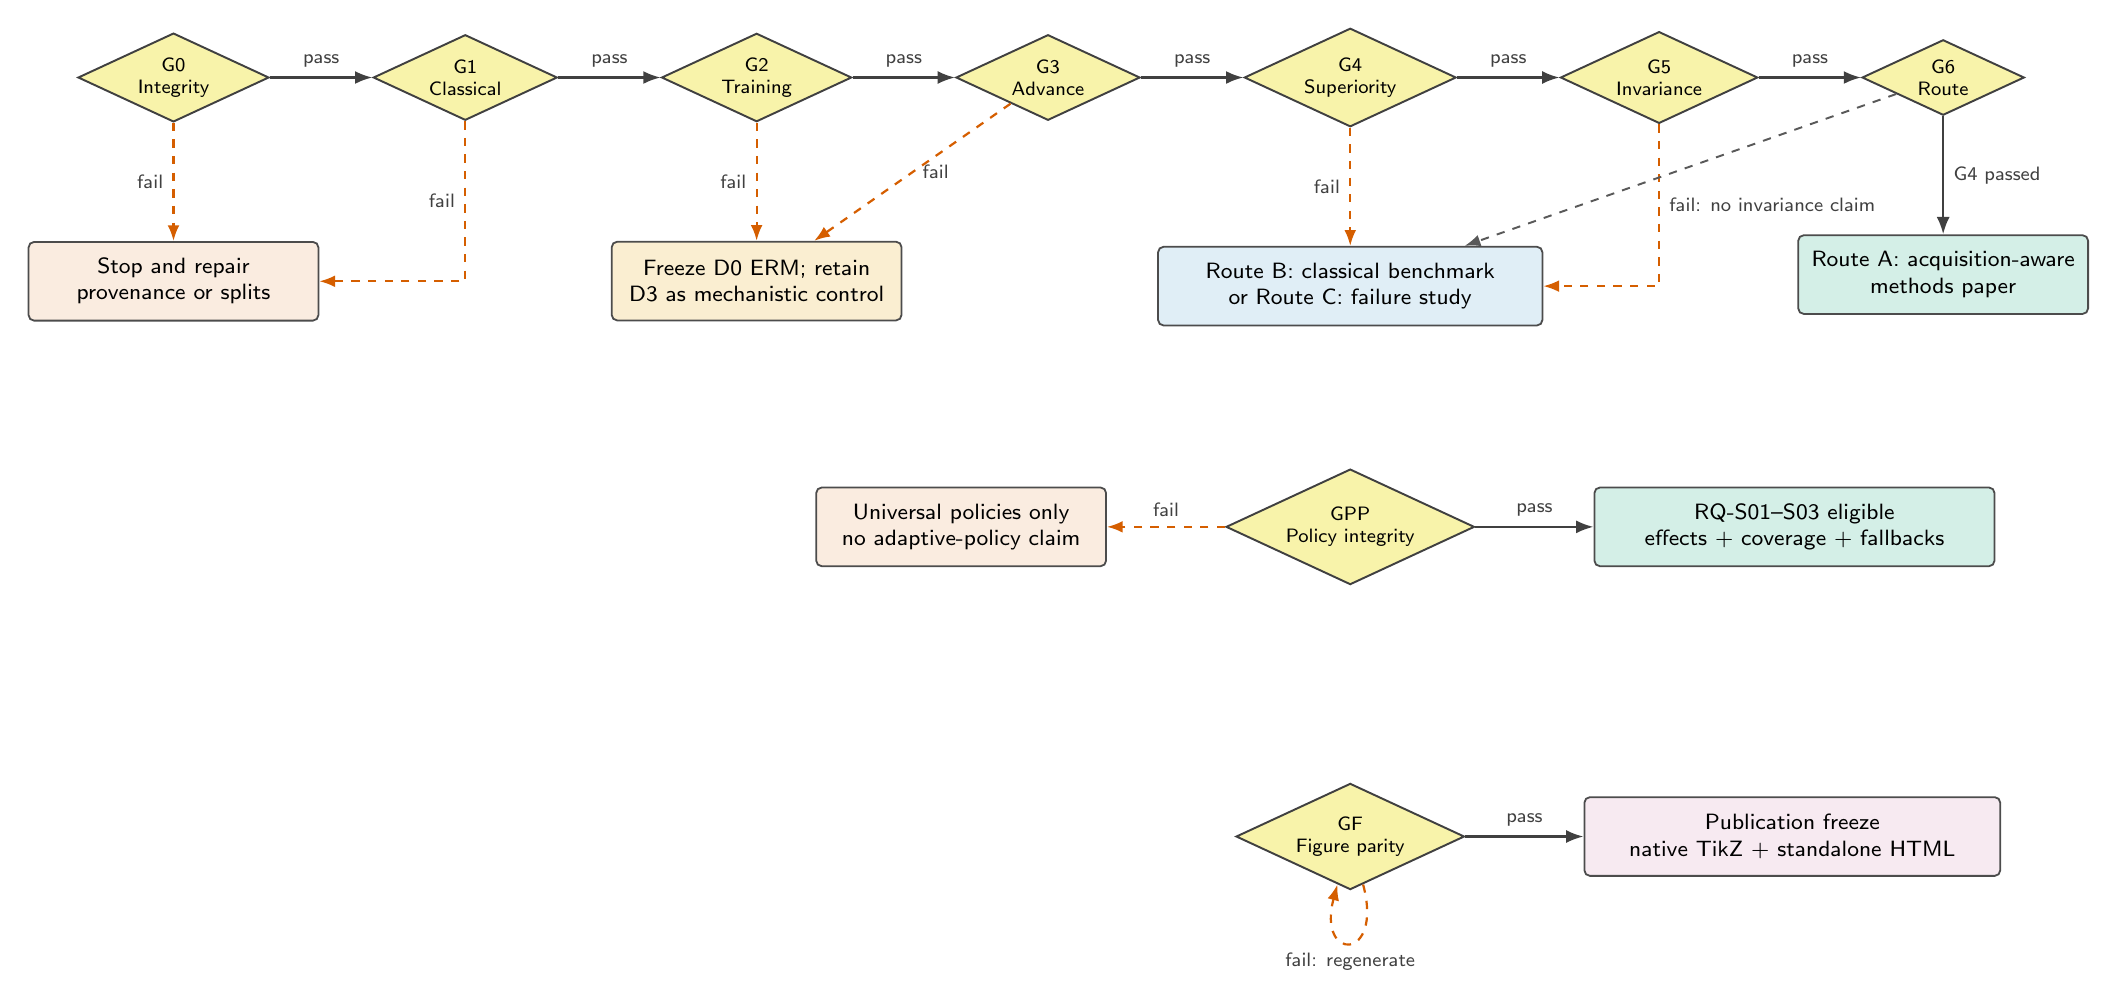
\begin{tikzpicture}[node distance=8mm and 13mm]
  \node[gate] (g0) {G0\\Integrity};
  \node[gate, right=of g0] (g1) {G1\\Classical};
  \node[gate, right=of g1] (g2) {G2\\Training};
  \node[gate, right=of g2] (g3) {G3\\Advance};
  \node[gate, right=of g3] (g4) {G4\\Superiority};
  \node[gate, right=of g4] (g5) {G5\\Invariance};
  \node[gate, right=of g5] (g6) {G6\\Route};

  \foreach \a/\b in {g0/g1,g1/g2,g2/g3,g3/g4,g4/g5,g5/g6}{
    \draw[flow] (\a) -- node[above,labeltext]{pass} (\b);
  }

  \node[planbox, fill=oiVermillion!12, below=15mm of g0] (stop) {Stop and repair\\provenance or splits};
  \node[planbox, fill=oiOrange!18, below=15mm of g2] (d0) {Freeze D0 ERM; retain\\D3 as mechanistic control};
  \node[planbox, fill=oiBlue!12, text width=46mm, below=15mm of g4] (routeb) {Route B: classical benchmark\\or Route C: failure study};
  \node[planbox, fill=oiGreen!17, below=15mm of g6] (routea) {Route A: acquisition-aware\\methods paper};

  \draw[failflow] (g0) -- node[left,labeltext]{fail} (stop);
  \draw[failflow] (g1) |- node[pos=.25,left,labeltext]{fail} (stop);
  \draw[failflow] (g2) -- node[left,labeltext]{fail} (d0);
  \draw[failflow] (g3) -- node[right,labeltext]{fail} (d0);
  \draw[failflow] (g4) -- node[left,labeltext]{fail} (routeb);
  \draw[failflow] (g5) |- node[pos=.25,right,labeltext]{fail: no invariance claim} (routeb);
  \draw[flow] (g6) -- node[right,labeltext]{G4 passed} (routea);
  \draw[secondaryflow] (g6) -- (routeb);

  \node[gate, below=18mm of routeb] (gpp) {GPP\\Policy integrity};
  \node[planbox, fill=oiVermillion!12, left=15mm of gpp] (ppfail) {Universal policies only\\no adaptive-policy claim};
  \node[planbox, fill=oiGreen!17, text width=48mm, right=15mm of gpp] (pppass) {RQ-S01--S03 eligible\\effects + coverage + fallbacks};
  \draw[failflow] (gpp) -- node[above,labeltext]{fail} (ppfail);
  \draw[flow] (gpp) -- node[above,labeltext]{pass} (pppass);

  \node[gate, below=25mm of gpp] (gf) {GF\\Figure parity};
  \node[planbox, fill=oiPurple!16, text width=50mm, right=15mm of gf] (freeze) {Publication freeze\\native TikZ + standalone HTML};
  \draw[flow] (gf) -- node[above,labeltext]{pass} (freeze);
  \draw[failflow, loop below] (gf) to node[below,labeltext]{fail: regenerate} (gf);

  % GPP is parallel to the primary G4 route: adaptive preprocessing can add a
  % secondary claim but cannot change the primary publication route.
\end{tikzpicture}
\end{document}
